In order to properly understand the \acs{rpnd}--the experimental measurements,
and the models, it is necessary to develop a theoretical underpinning. The
\acs{rpnd} is an ionized gas, and, dependent on its characteristics, a plasma.
Therefore, we begin with a review of the statistical description of an ionized
gas, equilibrium solutions, and several approximations. Subsequently, the
discharge initiation process is considered from the perspective of a single
avalanche. The Townsend model is briefly reviewed, followed by a more detailed
explanation of the streamer model. This naturally leads to the development of a
homogeneous discharge condition based on the preionization density--the basis
for the \acs{rpnd}. Following this, a qualitative introduction to atomic
structure is provided in order to introduce spectroscopic concepts such as
energy levels, transitions, lineshapes, and absorption cross sections.

\section{Ionized Gas}
An ionized gas is a volume of gas in which some fraction of the neutral atoms
and/or molecules have been separated into negative electrons and positive and/or
negative ions. For a sufficiently large number of particles and collision rate,
the behavior of each species in the ionized gas can be described by a continuous
distribution function.

This function is an expression of the likelihood of finding a particle within a
specific range of velocities in a specific volume, as a function of time. This
function is denoted as $f_\alpha(\vec{r}, \vec{v}, t)$, where the subscript
$\alpha$ denotes the species, $f$ is the distribution function, $\vec{r}$ is the
position, $\vec{v}$ is the velocity, and $t$ is the time.

The behavior of $f_\alpha$ can be shown \cite{Bellan2008} to be governed by the
Boltzmann equation,
\begin{equation}\label{eq:boltzmann}
  \frac{\partial f_\alpha}{\partial t} + \vec{v}\cdot\nabla f_\alpha +
  \frac{q_\alpha}{m_\alpha} \left(\vec{E} + \vec{v}\times\vec{B}\right)
  \cdot \nabla_v f_\alpha = \left( \frac{\partial f_\alpha}
  {\partial t}\right)_\mathrm{coll}.
\end{equation}
Here, $m$ is the particle mass, $q$ is its charge, $\vec{E}$ is the electric
field, $\vec{B}$ is the magnetic field, and $(\partial f_\alpha/\partial
t)_\mathrm{coll}$ is a term which represents changes to the distribution
function as a result of collisions. Coupled with Maxwell's equations,
equation~\ref{eq:boltzmann} provides a complete description of the behavior of
the fields and particles in a plasma.

For a species in equilibrium for no spatial gradients ($\partial f/\partial t =
\nabla f = 0$), it can be shown \cite{Druyvesteyn1940} that the distribution of
energies is
\begin{equation}\label{eq:mb}
  f_\alpha(\epsilon) = C \epsilon^{1/2}
          \exp\left( -\frac{\epsilon}{\kB T_\alpha}\right)
\end{equation}
where $C$ is a normalizing constant, $\epsilon$ is the energy, $\kB$ is
Boltzmann's constant, and $T_\alpha$ is the temperature of the species. This
equation referred to as the Maxwell-Boltzmann distribution. It should be
emphasized that this solution only applies when the classical species can be
considered to be in equilibrium. Gradients and electromagnetic fields can both
significantly alter the distribution function of a species. This can be of
particular importance in the calculation or reaction rates, or the measurement
of temperatures.

Additionally, the Boltzmann equation may be solved for electrons in equilibrium
with constant electric field, provided that a constant current density, and only
elastic collisions. Assuming that the mean free path of the electrons is
constant, the Druyvesteyn distribution may be defined as \cite{Druyvesteyn1940},
\begin{equation}
  f_\alpha(\epsilon) = C \epsilon^{1/2}
           \exp\left(-\frac{\epsilon^2}{\langle \epsilon \rangle^2} \right)
  \label{eq:druy}
\end{equation}
where $\langle\epsilon\rangle$ is some mean energy, determined by the gas
properties. This solution tends to suppress the probability of higher and
lower-energy electrons in favor of more intermediate values.
Figure~\ref{fig:simpledists}
\begin{figure}
  \centering
  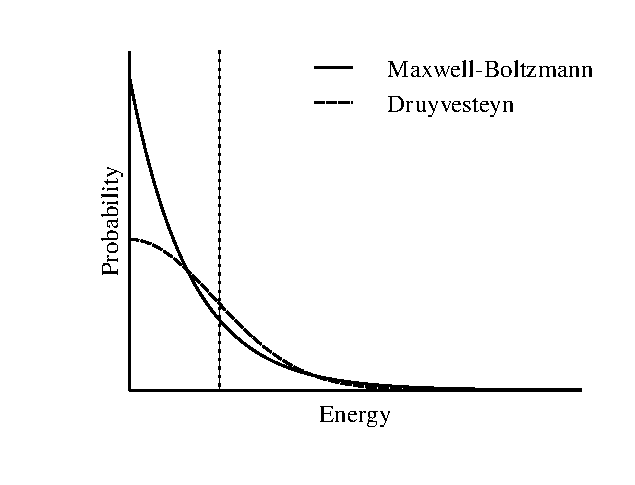
\includegraphics{./chapters/theory/figures/simpledists.eps}
  \caption{Comparison of the Maxwell-Boltzmann energy distribution and the
    Druyvesteyn distribution for the same average energy (illustrated by the
  dotted line).}
  \label{fig:simpledists}
\end{figure}
compares the probability distributions from equations~\ref{eq:mb}
a]nd~\ref{eq:druy} for the same temperature $T_\alpha$. The dotted line
illustrates the average energy for the two distributions, which is not the same
as the most probably energy.

Additional solutions of equation~\ref{eq:boltzmann} in anything but these simple
cases can be very challenging (c.f.\ Chapter 18 of \cite{Lieberman2005}). Even
computational approaches can be stymied by the seven-dimension phase space and
high dynamic range. In most situations, the Boltzmann equation is converted to
more tenable expressions by integrating it over velocity-space. The first
so-called moment is the conservation equation or continuity equation
\cite{Lieberman2005},
\begin{equation}\label{eq:cont}
  \frac{\partial n_\alpha}{\partial t} + \nabla \cdot (n_\alpha \vec{u_\alpha})
  = G_\alpha - L_\alpha.
\end{equation}
In this case, there is now a mean velocity $\vec{u}$, as well as gain ($G$) and
loss ($L$) terms which replace the collision operator. The gain and loss terms
are generally expressed as the product of the densities of the interacting
species, and a rate coefficient. For an electron-impact interaction where the
target is relatively stationary, the rate coefficient is
\begin{equation}
  K = \int_0^\infty f_e(\epsilon)\sigma(\epsilon)
      \sqrt{\frac{2\epsilon}{m_e}}d\epsilon,
  \label{eq:rate}
\end{equation}
where $\sigma$ is the energy-dependent cross section.

The definition of the mean velocity, $\vec{u}$ can be obtained by multiplying
equation~\ref{eq:boltzmann} by $v$ and integrating over velocity-space, to
obtain the second moment \cite{Lieberman2005},
\begin{equation}
  m_\alpha n_\alpha \left[ \frac{\partial \vec{u_\alpha}}{\partial t}
  + (\vec{u_\alpha} \cdot \nabla) \vec{u_\alpha}\right]
  = q_\alpha n_\alpha (\vec{E} + \vec{u_\alpha} \times \vec{B})
  - \nabla \cdot \vec{\Pi} + \vec{f}|_\mathrm{coll}.
  \label{eq:momentum}
\end{equation}
This expresses the conservation of momentum by the plasma. It provides a means
by which to solve for the mean velocity of the system, however it also
introduces two additional terms. $\vec{f}|_\mathrm{coll}$ deals with the forces
transferred to $\alpha$ via collisions. This term is often approximated as the
Krook collision operator, which is only dependent on known quantities: $m$, $n$,
$\vec{u}$, $G$, $L$, and the momentum transfer frequency, $\nu_\mathrm{m}$, for
the species $\alpha$ and all species it interacts with. The second term,
$\vec{\Pi}$, is the pressure tensor and can only be defined by the third moment
of the Boltzmann equation. In fact, each additional moment introduces a new term
requiring a higher order moment, \emph{ad infinitum}. In most situations, this
chain of equations is terminated after the first two or three moments by the use
of an additional assumption such as an equation of state.

For the purposes of this paper, one more moment will suffice. Assuming that the
pressure is isotropic, one can multiply equation~\ref{eq:boltzmann} by $mv^2/2$,
and integrate over velocity-space to find the energy conservation equation,
\begin{equation}
  \frac{\partial}{\partial t}\left(\frac{3}{2}p_\alpha\right) 
  + \nabla\cdot\frac{3}{2} (p_\alpha\vec{u}_\alpha)
  + p_\alpha\nabla\cdot\vec{u}_\alpha
  + \nabla\cdot\vec{q}_\alpha
  = \frac{\partial}{\partial
  t}\left(\frac{3}{2}p_\alpha\right)\bigg|_\mathrm{coll}.
  \label{eq:energy}
\end{equation}
In this case, $p$ represents the isotropic pressure, and $\vec{q}$ is the heat
flow. The first term on the LHS represents the total energy contained by the
species, the second term is the energy flux in and out of the volume, and the
third term accounts for changes due to compression or expansion. The RHS is the
collision operator which describes energy added or removed from the system as a
result of collisions.

Equations~\ref{eq:cont} and~\ref{eq:energy} are particularly important for this
study. As will be detailed in Chapter~\ref{chp:modeling}, the two can be used to
create a global model of the plasma. Such a model assumes spatial homogeneity of
the plasma in order to reduce the associated computational costs. This allows
the model to address large numbers of species over long periods of time as will
be required in the case of the \acs{rpnd}.

\section{Plasma Criteria}
Though the Boltzmann equation describes both an ionized gas and a plasma, the
two are distinct as a plasma is necessarily an ionized gas, but not vice versa.
A plasma is unique in that its dynamics are governed by long range
electromagnetic forces, unlike gases in which short-range collisions dominate.
As a result, plasmas frequently exhibit large scale structure and organization.
Examples of these structures are ubiquitous in astronomy where phenomena such as
the aurora borealis, coronal mass ejections, and even interstellar media are all
plasmas \cite{Chen1984}. There are three criteria which form a more exact
definition of what constitutes a plasma.

\subsection{Debye Length}
If an electrical perturbation is introduced into an ionized gas, the charged
particles will tend to rearrange themselves to shield it out. A plasma is an
ionized gas which is large enough for this shielding effect to occur. The
characteristic length scale for this shielding effect to take place is referred
to as the Debye length, denoted $\lambda_D$. It can be shown to be equal to
$\sqrt{\epsilon_0T_e/(en_0)}$, where $\epsilon_0$ is the vacuum permittivity,
$T_e$ is the electron temperature, and $n_0$ is the plasma density. If the
characteristic length scale of the ionized gas is $L$, then $\lambda_D < L$ for
it to be considered a plasma.

\subsection{Debye Sphere}
However, the above condition by itself is not sufficient for shielding to occur.
It is possible that an ionized gas may have a relatively small Debye length, but
also lack enough charged particles for shielding to occur. More simply put, it
would be impossible for a single electron to shield out even the smallest of
perturbations. For that reason, the number of particles in a Debye sphere must
be greater than unity in a plasma, or $n_0(4\pi \lambda_D^3/3) >>
1$.\footnote{This condition is also implied in the derivation of the Debye
length.}

\subsection{Plasma Oscillations}
Finally, a plasma may exhibit Debye shielding, but lack collective motion of the
charged particles. This can occur when the collision frequency with neutral
particles is too high. In this case, the behavior of the ionized gas is
significantly affected by random collisions. Therefore, the characteristic
response frequency of a plasma, commonly called the plasma frequency, should be
greater than the neutral collision frequency ({$\omega_p > \nu$}) in order for
this collection motion to occur. The plasma frequency can be shown to be
$\omega_p = \sqrt{e^2n_0/(\epsilon_0 m_e)}$ \cite{Chen1984}.

There are many natural and man-made plasmas of varying size and quality.
Figure~\ref{fig:regimes}
\begin{figure}
  \centering
  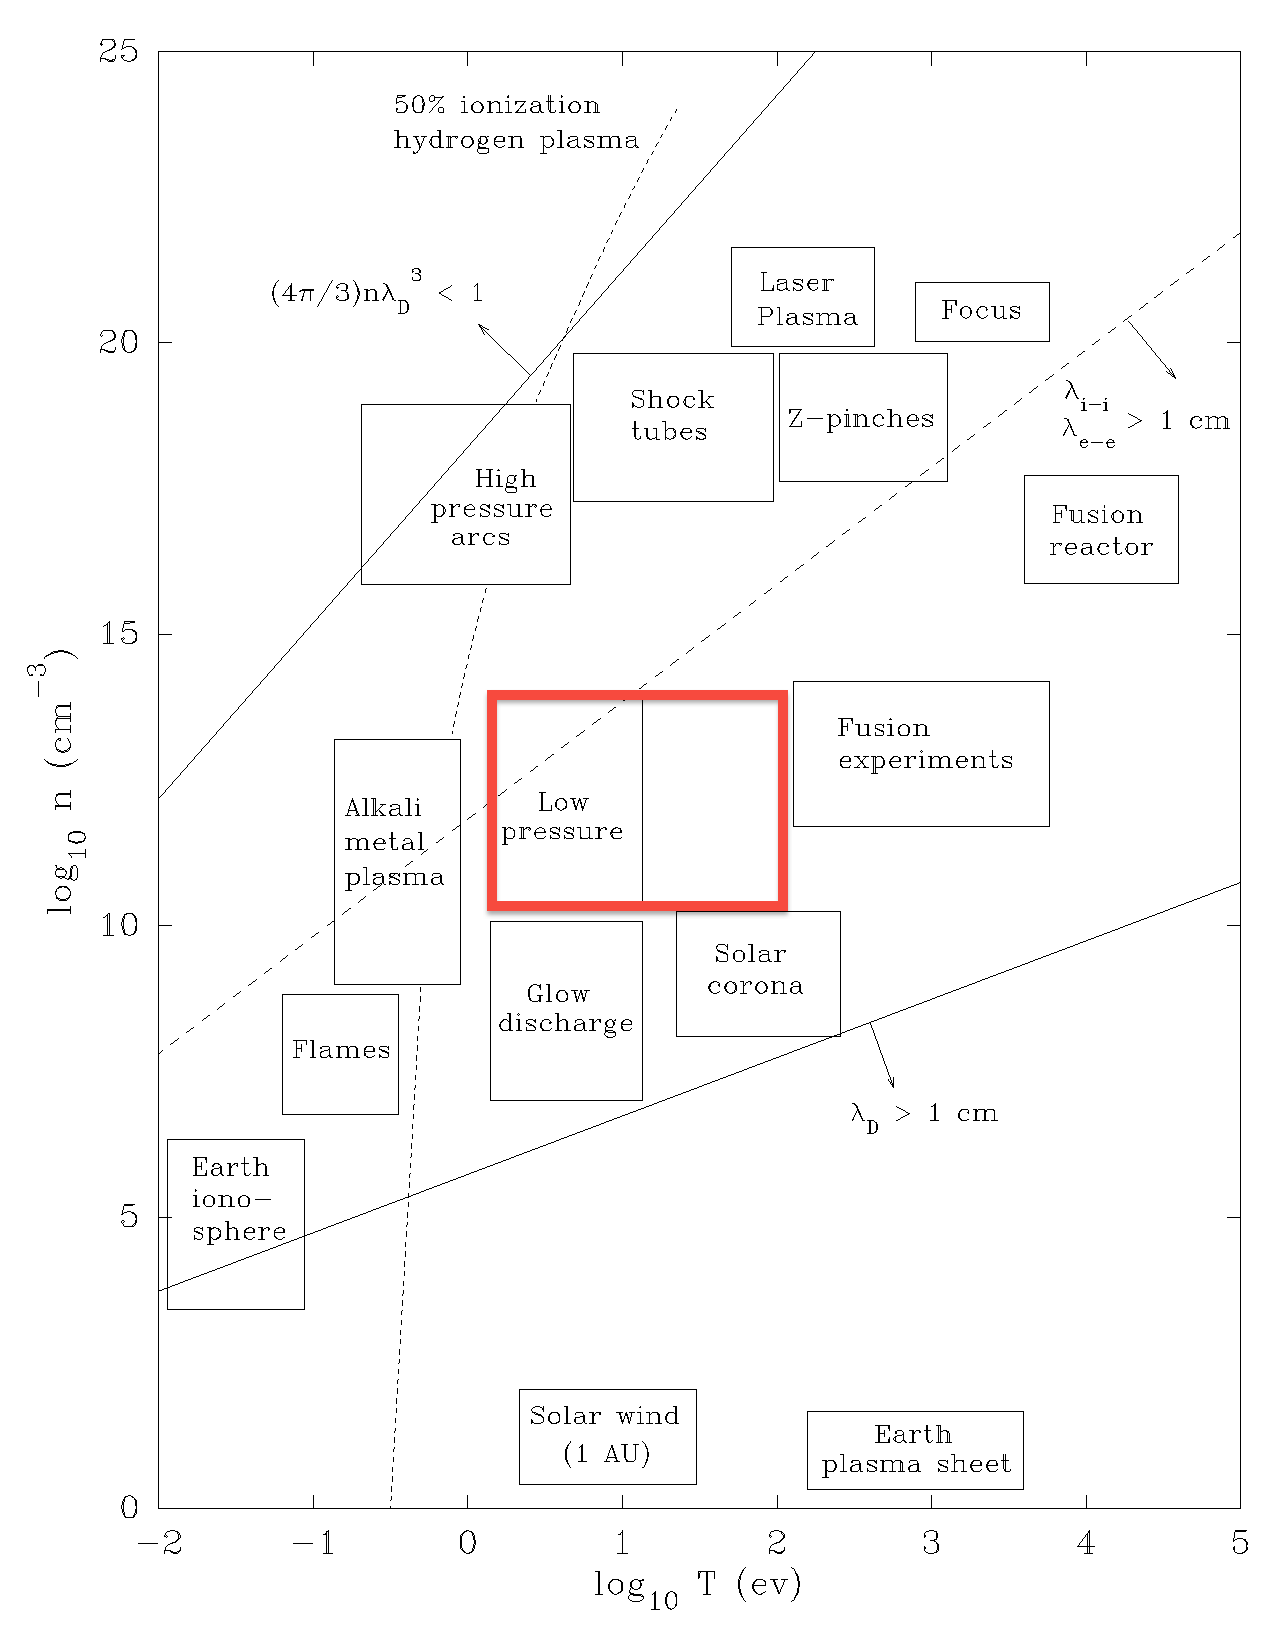
\includegraphics{./chapters/theory/figures/regimes.pdf}
  \caption{Illustration of the various regimes of plasma in terms of
    electron temperature and density with the \acs{rpnd} regime highlighted,
    adapted from \cite{Huba2011}.}
  \label{fig:regimes}
\end{figure}
shows several categories of plasma, plotted as a function of their electron
density and temperature. As can be seen in this example, the electron densities
span seven decades, and the densities cover in excess of 20. This broad range of
conditions presents a particularly challenging problem for both simulations and
experimental measurements. Also highlighted in the figure is the range spanned
by the \acs{rpnd}.

\section{Discharge Initiation}
The Boltzmann equation is a continuous, statistical description of a plasma. By
comparison, the initial breakdown of a plasma is a highly discontinuous process
marked by its stochasticity. The initiation of a discharge is typically the
result of electron avalanches which occur randomly throughout a volume of gas
\cite{Druyvesteyn1940}. Often, the seed electrons for a plasma are the products
of ionizing cosmic rays. At sea level this results in a few electrons per
cubic-centimeter. As a result, it is necessary to consider the initiation of a
discharge separately from a pre-existing plasma.

\subsection{Townsend Mechanism}

Classically, plasmas are created by two different mechanisms, the applicability
of which depends on primarily on the strength of the electric field relative to
the neutral gas density, a value called the reduced electric field
\cite{Huxley1966}. At lower reduced fields, the Townsend mechanism is
responsible for the formation of a plasma. Consider two electrodes separated by
a gap filled with some gas. An electron starting near the cathode will drift
toward the anode. For a large enough electric field, the electron will gain
sufficient kinetic energy to ionize a neutral atom, producing a second electron.
The two electrons are now accelerated by the field, instigating further
ionization of the background gas. The population of electrons quickly grows,
thus the process is referred to as an electron avalanche. Eventually, the
avalanche electrons are collected at the anode.

In their wake are ions which slowly drift toward the cathode. As the ions impact
the surface of the cathode, they occasionally cause a secondary electron to be
emitted. This secondary electron initiates a new avalanche and helps to sustain
the discharge. A steady state electric discharge occurs when the current of the
ion collection at the cathode matches the current of the electron collection at
the anode. The time scale of the Townsend discharge is usually determined by the
positive ions, as their large mass results in slow drift velocities. For an
electric field of 50 V/cm at 200 mTorr, the drift velocity of a helium ion in
helium is about $7\times10^4$ cm/s \cite{Hornbeck1951}. For a gap of 10 cm, this
gives a drift time on the order of $10{-4}$ s.

The Townsend mechanism is characterized by two parameters: $\alpha$ and
$\gamma$, the first and second Townsend coefficients. $\alpha$ is the number of
ionization events that occur per unit length, often expressed as a function of
the reduced field \cite{Druyvesteyn1940}. The second Townsend coefficient is the
probability that an ion impinging on the cathode produces a secondary electron.
The values for $\gamma$ can vary widely and depends on the type of ion, its
energy, the cathode material, contamination of the surface, and many other
factors. That said, typical values are around 0.01-0.1 \cite{Lieberman2005}.

\subsection{Streamer Mechanism}

In contrast, the streamer discharge which occurs for larger values of the
reduced field does not depend on secondary emission. Additionally, streamer
discharges can develop in time periods as short as 1 ns, much less than the time
required for Townsend breakdown. In order to describe the streamer mechanism,
again consider an electron between two electrodes, as seen in (a) of
figure~\ref{fig:streamer}.
\begin{figure}
  \centering
  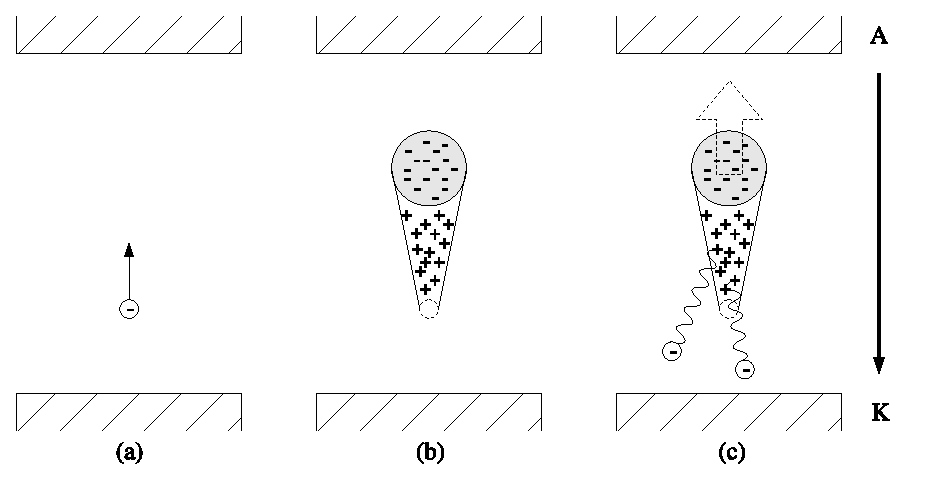
\includegraphics{./chapters/theory/figures/streamer.eps}
  \caption{An illustration of the development of a single streamer. (a)
    A seed electron is accelerated by the applied electric field. (b) The
    initial electron develops into an avalanche which leaves a large region
    of positive space charge, slowing further advance. (c) The streamer
    propagates toward the cathode via photoionization and the anode via
    nonlocal electrons and photoionization. Adapted from \cite{Levatter1980} and
    \cite{Kunhardt1980}.}
  \label{fig:streamer}
\end{figure}
As with the Townsend discharge, this electron initiates an avalanche which moves
toward the anode. As the electrons travel toward the anode, they randomly
collide and diffuse, leaving behind a cone of ions, as seen in part (b).
However, the higher reduced field drastically increases $\alpha$. This causes
the space charge of the avalanche to create an electric field comparable to the
one that is applied, slowing the propagation of the avalanche.

At this point the avalanche can be considered a streamer as it begins to
increase its extent by several additional processes. The large internal fields
of the avalanche can accelerate individual electrons and ``inject'' them in the
direction of the anode \cite{Kunhardt1980}. In addition, as the excited atoms in
the wake of the avalanche begin to radiate, they can cause photoionization
throughout the volume. Photoelectrons generated close enough to the negative
head, or positive tail of the streamer will initiate secondary avalanches which
eventually connect to the primary one. While photoelectrons may cause some
additional broadening of the streamer, the injection of electrons toward the
anode is aligned with the direction of the internal field of the avalanche. As a
result, the ionization caused by these electrons do not appreciably increase the
radius of the streamer.

\subsection{Homogeneity Condition}

However, these processes are not critical in the formation of a large-volume
discharge by an \acs{rpnd}. This description of a streamer only considers an
avalanche generated by a single electron. In reality, many can form
simultaneously assuming that there is more than one seed electron in the volume.
With moderate preionization of the volume, the strong fields of the individual
avalanches can begin to overlap\footnote{If the preionization of the volume is
too large, it can effectively short out the electric field.}. This smoothes out
the field gradients which would otherwise radially constrict the streamers.
Instead, ionization progresses homogeneously throughout the volume.

In order to determine the necessary preionization density, we refer to the work
done by Levatter and Lin on gas laser discharges \cite{Levatter1980}. First, the
electron drift velocity in an applied field can be expressed as the product of
the field and the electron mobility $\mu$. The electron mobility multiplied by
the electric field is the steady-state drift velocity for an electron in that
field and represents the balance between the frictional force of the neutral gas
collisions and the electric field. Consequently, the mean velocity of electrons
drifting in a time-varying field $E(t)$ can be expressed as
\begin{equation}
  u(t) = \mu(E) E(t).
\end{equation}

The length of the avalanche can be written as a time-integrated function of the
electron drift velocity,
\begin{equation}
  \xi = \int_{t_0}^t u(t) dt.
  \label{eq:s_xi}
\end{equation}
Here, $t_0$ is the time at which $E(t)$ becomes high enough that the first
Townsend coefficient, $\alpha$, exceeds 0. Because no electron multiplication
occurs while $\alpha < 0$, this effectively represents the beginning of the
avalanche.

The electric field in the head of the avalanche depends on its radius, which is
dependent on the diffusion of the electrons as they cross the gap. This is
governed by the free diffusion coefficient, $D$. For a fixed diffusion constant,
the final avalanche radius would simply be $R = \sqrt{2D\Delta t}$, where
$\Delta t$ is the time after breakdown. As the diffusion coefficient typically
varies with the applied electric field, the final avalanche radius will be
assumed to be equal to $R = \sqrt{2\bar{D}\Delta t}$, where $\bar{D}$ is the
time-averaged diffusion coefficient.

Levatter and Lin assume that the avalanche slows when the peak field of the
avalanche is equal to the applied field. Assuming that the electrons diffuse
equally in all directions, the electric field of the avalanche head can be
expressed as
\begin{eqnarray}
  E_a(r) = \frac{eN_e}{4\pi\epsilon_0R^2} F(r/R), \qquad \mathrm{where} \\
  F(r/R) = \frac{1}{R^2}\left[\mathrm{erf}(r/R)-\frac{2}{\pi^{1/2}}
           (r/R)\exp(-r^2/R^2)\right] ,
\end{eqnarray}
where $r$ is the radius with respect to the center of the avalanche, $N_e$ is
the number of electrons in the avalanche, $\mathrm{erf}$ is the error function.
$F$ is a dimenionless function which has a peak value of $0.428$. Provided
$\alpha$ as a function of reduced field, the number of electrons in the
avalanche is equal to
\begin{equation}
  N_e = \int_0^\xi \alpha(\xi')d\xi'.
  \label{eq:s_pop}
\end{equation}

Here, Levatter and Lin make a number of assumptions in order to develop an
analytic and dimensionless solution for $E_{a,\mathrm{max}}(t) = E(t)$. However,
it is possible to numerically integrate equations~\ref{eq:s_xi}
and~\ref{eq:s_pop} to determine the time required for the avalanche to slow.
This should provide a more accurate, but less general result. Assuming a
linearly increasing electric field, figure~\ref{fig:avalanche_lengths}
\begin{figure}
  \centering
  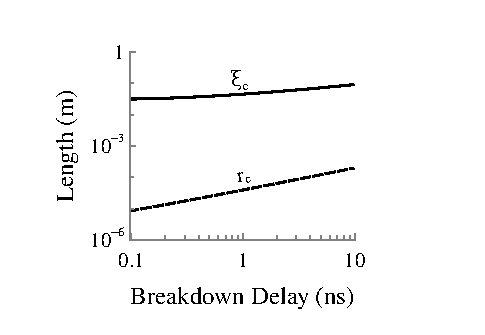
\includegraphics{./chapters/theory/figures/avalanche_lengths.eps}
  \caption{Numerical calculations of the avalanche length and avalanche radius for
    in helium at a pressure of 4.0 Torr as a function of the time required for
    $\alpha > 0$ to occur (based on a fixed electric field slope).}
  \label{fig:avalanche_lengths}
\end{figure}
shows the results of such calculations for an avalanche in 4.0 Torr of helium,
as a function of various breakdown delays (final field strengths ranged from
40-143 Td). The breakdown delay is defined as the time it takes for $\alpha >
0$. The mobilities, diffusion coefficients, and Townsend coefficients were
interpolated from solutions of the Boltzmann equation provided by the BOLSIG+
code with Phelps' cross sections \cite{Phelps2002}. For this range of breakdown
delays, the avalanche was able to develop up to nearly 10 cm in length before it
slowed. The times required for the avalanche to slow ranged from around 23 ns
for the shortest breakdown delay, and 389 ns for the longest.

From this, a criteria for homogeneous breakdown of the gas can be developed. In
order for the field gradients to be smoothed out, the individual avalanche heads
should roughly overlap by the time they have slowed. Assuming that all seed
electrons in the volume initiate avalanches, this can be approximated as
$n_{e,c} > r_c^{-3}$, where $n_{e,c}$ is the critical electron density, and
$r_c$ is the avalanche radius when it has slowed. As seen in
figure~\ref{fig:avalanche_densities},
\begin{figure}
  \centering
  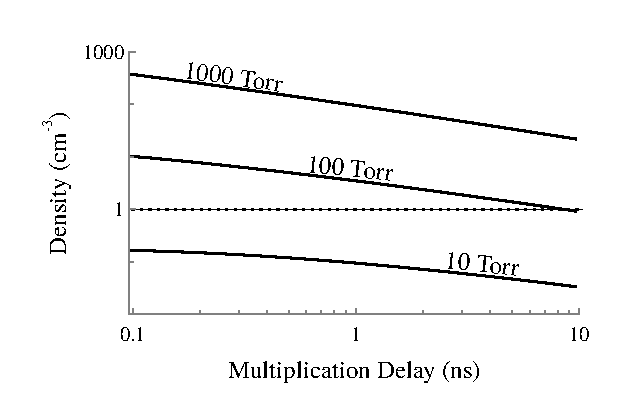
\includegraphics{./chapters/theory/figures/avalanche_densities.eps}
  \caption{Minimum preionization densities required at a variety of pressures
    and delays before the $\alpha > 0$ is reached. The dotted line indicates the
    background ionization level as a result of cosmic radiation.}
  \label{fig:avalanche_densities}
\end{figure}
the required preionization density depends on both the breakdown delay and the
operating pressure. Generally, the preionization density increases with pressure
and decreases with breakdown delay. The dotted line in the figure indicates the
anticipated background electron density from cosmic radiation. This suggests
that, for the breakdown delays in question, the discharge will almost always be
homogeneous at pressures below 100 Torr. While the plot suggests that large
values of $dE/dt$ might guarantee homogeneous breakdown at near-atmospheric
pressure, the increasing likelihood of ionization instabilities \cite{Johns1972}
will preclude homogeneous discharge development.

\section{Atomic Spectroscopy \& Notation}

As described, much of the experimental work presented will concern the use of
spectroscopic techniques. Careful measurements of the light emitted from excited
atomic states can yield electron densities and temperatures, excited state
densities and temperatures, electric fields, and magnetic fields
\cite{Griem2005}. The topic of spectroscopy is extensive and it is neither
necessary nor desirable to cover it in full. Instead we will only consider what
is necessary to understand the emissions from a singly-excited, multi-electron
atom.

An atom is composed of a small, positively charged nucleus, orbited by
negatively charged electrons. The actual position of any single electron is
probabilistic and described by a wavefunction--solutions of the Schr\"{o}dinger
equation for the atom in question. Each wavefunction is associated with a number
of eigenvalues which quantize aspects of the state of bound electrons. In simple
atoms, four such quantum numbers are of interest \cite{Drake2006},
\begin{itemize}
  \item $n=1,2,\ldots$: the principal quantum number,
  \item $l=0,1,\ldots,n-1$: the orbital angular momentum number,
  \item $m_l =-l,\ldots,l$: the projection of $l$, and
  \item $m_s=\pm1/2$: the projection of the spin quantum number.
\end{itemize}
The quantum numbers are hierarchical such that each $n$, or shell, possesses a
series of subshells, $l$, while each subshell possesses a number of individual
orbital, $m_l$, and each orbital possess one of two spins. As a result of the
Pauli exclusion principle, the wavefunction of each electron around an atom is
described by a \emph{unique} set of quantum numbers. This means, that any
particular subshell can only contain $2(2l+1)$ electrons. The subshells are
often referred to using the nomenclature $0,1,2,3,\ldots = s,p,d,f,\ldots$.

As a result of their separation from the nucleus, the electrons in an atom
possess some degree of potential energy. As the $n$ and $l$ of an electron
increase, so does its potential energy. In the absence of electric and magnetic
fields, $m_l$ and $s$ do not affect the potential energy of an electron. As an
example, an electron in the 1s ($n=1$ and $l=0$) subshell has the lowest
possible potential energy.

Absent from external influences, the individual states are populated with
electrons so as to minimize the total potential energy of the system. This
natural arrangement is referred to as the ground state configuration. Often, but
not always, the subshells are filled sequentially and in order from lowest to
highest $l$ \cite{Drake2006}. Provided some input energy in the form of a
collision or a photon, one or more of the electrons surrounding the atom may
transition to another state, increasing the potential energy of the system. In
low-temperature plasmas it usually one of the electrons from the outermost or
partially filled subshell to be excited.

The potential energies of the electron configurations for multi-electron atoms
are determined by the collective effects of all the surrounding electrons.

It is the collective effects of all electrons surrounding an atom which
determine its potential energy. This results in a single set of total angular
momenta which can be used to describe the atom. In lighter atoms
\cite{Drake2006}, the contributions of the individual electrons are combined
assuming a condition called L-S coupling. Under this assumption, the total
angular momentum of the atom can written as $\vec{L} = \sum\vec{l}_i$, where $i$
is each electron in a partially filled subshell (filled subshells sum to zero).
Likewise, the total spin can be written as $\vec{S} = \sum\vec{s}_i$. These can
be combined to form the total angular momentum of the atom, $\vec{J} = \vec{L} +
\vec{S}$. Finally, the each atom is said to have an even or odd parity, defined
as $(-1)^{\sum\bm{l}_i}$, where $-1$ is odd, and $1$ is even.

These quantities can be used to write a ``term symbol'' for the atom, of the
form $^{2S+1}L_J^p$, where $p$ is `o' if the parity is odd, and omitted if it's
even. The term symbol can be augmented by prepending additional terms which
address the subshells in which electrons can be found. This is typically written
as $nl^N$, where $N$ is the number of electrons in a given subshell (ommitted if
$N=1$). For example, 1s2s$^3$S$_{1}$, describes the triplet helium metastable
state. In this case, there is a single electron in the 1s subshell and a second
atom in the 2s subshell. The configuration has a total orbital angular momentum
of 0 (denoted by the `S'), an even parity (denoted by the absence of a
superscript `o'), a total spin of $1$ (the superscript $3$ is equal to $2S+1$),
and a total angular moment of 1.

Excited atomic states usually have finite lifetimes. Normally, electrons will
undergo transitions to lower the potential energy of the system. This can also
occur spontaneously, through the emission of a photon, or through a superelastic
collision with another particle. In the case of spontaneous transitions, only
certain states can transition to others, as defined by a series of selection
rules \cite{Drake2006}:
\begin{itemize}
  \item $\Delta S = 0$
  \item $\Delta L = \pm1$ or 0
  \item $\Delta J = \pm1$ or 0
  \item $L=0$ cannot transition to $L=0$
  \item $j=0$ cannot transition to $J=0$
\end{itemize}
These rules are determined from a lower order approximation, and thus are not
strict. As a result, forbidden transitions can occur, however these generally
take place at much lower rates.

Figure~\ref{fig:grotrian}
\begin{figure}
  \centering
  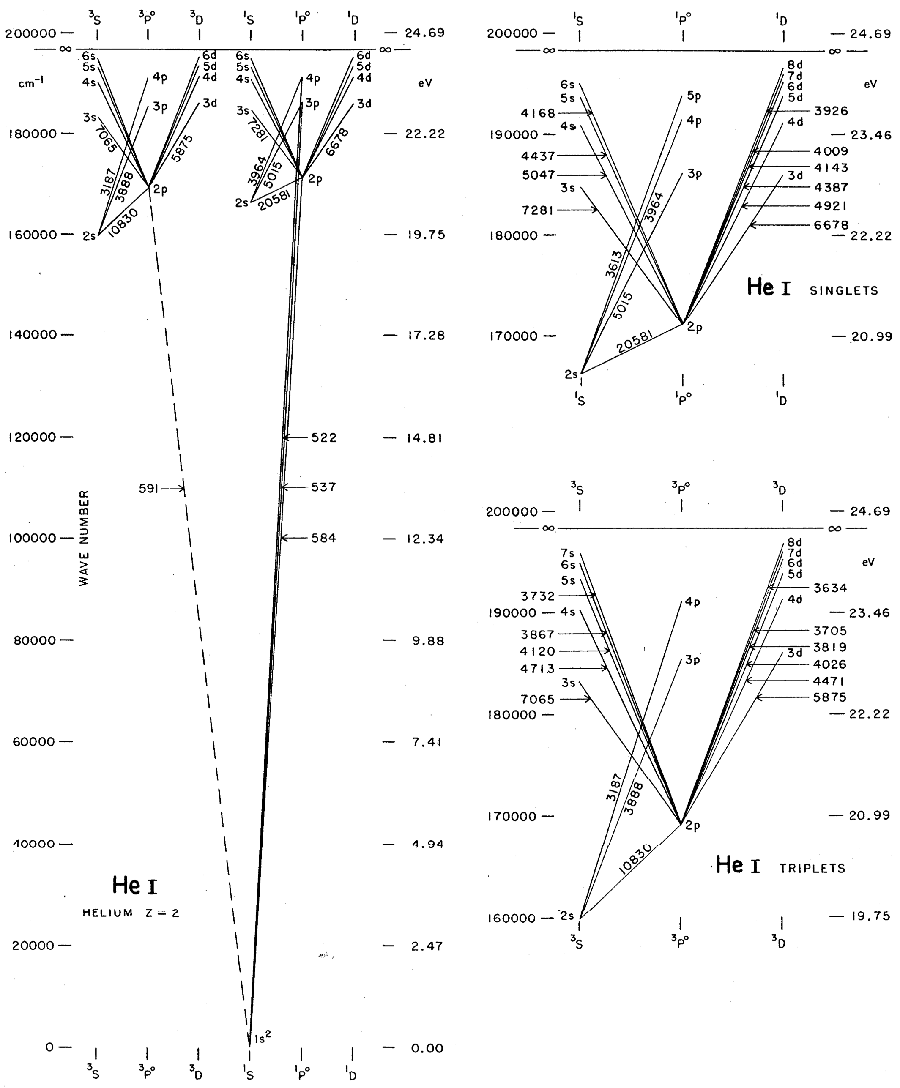
\includegraphics{./chapters/theory/figures/grotrian.pdf}
  \caption{A partial Grotrian diagram of neutral helium, from \cite{Moore1968}.}
  \label{fig:grotrian}
\end{figure}
is a Grotrian diagram of the energy levels in neutral helium and the allowed
transitions. In this case, the atomic states are separated into the singlet
($S=0$) and triplet ($S = 1$) manifolds. The singlet manifold is composed of
excited states where the electron spins are anti-parallel, and the triplet
manifold represents excited states where the electron spins are parallel. As
indicated by the first selection rule, transitions between these two manifolds
is forbidden, thus each is something of a self-contained system
\cite{Herzberg1944}.

Also observable in the diagram are two ``metastable'' states. These are the 2s
states at the bottom of the singlet and triplet manifolds. An electron in either
state cannot spontaneously transition to a lower energy state. As a result, an
electron in either state can be extremely long-lived. In addition, they are also
the lowest-lying excited states of helium. For these reasons, helium plasmas
tend to have high densities of metastable atoms. This makes them a good
candidate for spectroscopic study as will be seen in
Chapter~\ref{chp:metastables}.

\subsection{Spectral Lineshapes}

Electrons which transition to lower energy states emit photons which can be
detected. Conversely, if an atom is exposed to a photon with an energy matching
a transition, the atom may absorb the photon. Both processes are useful in
determining the prevalence and dynamics of the excited states. This, in turn,
can be used to infer various plasma properties.

Conservation of energy requires that the energy of the absorbed or emitted
photon match the energy difference between the two states. However, the finite
lifetime of excited atomic states implies, via the time-energy formulation of
the uncertainty principle, some uncertainty in the actual energy difference
between the states. As a result, the emitted photon will possess an energy
selected from a distribution of energies.

This distribution is referred to as the spectral lineshape. The narrowest
permissible lineshape, or natural lineshape, of an atomic transition can be
shown \cite{Siegman1986} to be a Lorentzian of the form,
\begin{equation}
  g(\omega) = -\frac{1}{4\pi^2}\frac{A\lambda^3}{\dwa}
  \frac{1}{1 + \left[2(\omega-\omega_a)/\dwa\right]^2},
  \label{eq:lorentzian}
\end{equation}
where $\omega$ is the photon frequency, $A$ is the Einstein coefficient for the
transition, $\lambda$ is the wavelength of the transition, $\omega_a$ is central
frequency of the transition, and $\dwa$ the full-width half maximum (\acs{fwhm})
of the transition. In the ideal case, where the atoms motionless and unaffected
by external perturbations, $\dwa = A$ \cite{Siegman1986}. This is known as the
natural linewidth.

Other processes can act to broaden or alter the spectral lineshape
\cite{Kunze2009}. For example, inter-atomic collisions can reduce the lifetimes
of excited states. This results in additional broadening of the line, though it
retains its Loretnzian nature. As the frequency of inter-atomic collisions
increases linearly with pressure, this phenomena is referred to as pressure
broadening. It can be included in equation~\ref{eq:lorentzian} by using $\dwa =
A + BP$, where $B$ is a measured or calculated broadening coefficient, and $P$
is the pressure \cite{Siegman1986}.

Atomic motion can also play a role in the spectral lineshape. If an atom is
moving toward or away an observer as it emits a photon, the emitted photon will
be blue or red shifted. Likewise, if the atom is moving toward or away an
incident photon, the energy of that photon will be shifted \cite{Siegman1986}.
If this effect is averaged over the random motion of atoms in a gas, the result
is an additional broadening of the lineshape, called Doppler broadening. Unlike
pressure broadening, Doppler broadening introduces a Gaussian component to the
lineshape such that,
\begin{multline}
  g(\omega) = \sqrt{\frac{2\ln{2}}{\pi^3}}\frac{\dwa}{\dwd}
  \int_{-\infty}^\infty
  \frac{1}{[(\omega - \omega_a) - \omega']^2 + 4\dwa^2} \\
  \times \exp\left[4\ln{2}\left(\frac{\omega'}{\dwd}\right)^2\right]d\omega'.
  \label{eq:voigt}
\end{multline}
Here, $\dwd = \omega_a\sqrt{\frac{8k_\mathrm{B}T_\mathrm{g}\ln{2}} {Mc^2}}$, is
the width of the Doppler broadening, where $T_g$ is the gas temperature, $M$ is
the particle mass, and $c$ is the speed of light. This form of the spectral
lineshape is known as the Voigt profile, and it must be numerically integrated.
In the case that $\dwd >> \dwa$, equation~\ref{eq:voigt} can be simplified to a
standard Gaussian distribution,
\begin{equation}
  g(\omega) = \sqrt{\frac{4\log{2}}{\pi\dwd^2}}
  \exp\left[-(4\log{2})\left(\frac{\omega-\omega_a}{\dwd}\right)^2\right].
\end{equation}

The effect of the various broadening mechanisms is most apparent in the wings of
the lineshape, far from the peak. Figure~\ref{fig:lineshapes}
\begin{figure}
  \centering
  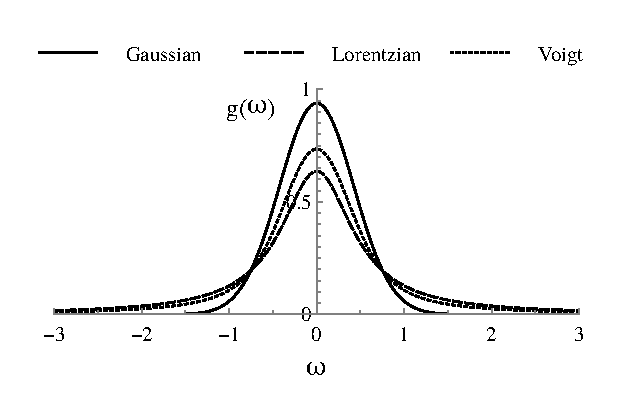
\includegraphics{./chapters/theory/figures/lineshapes.eps}
  \caption{A comparison of the three primary spectral lineshapes, each with the
  same full width.}
  \label{fig:lineshapes}
\end{figure}
illustrates the three major lineshapes with equivalent full widths. The Voigt
profile is composed of equally broad Lorentzian and Gaussian distributions. As
can be seen, the wings of the Gaussian distribution fall off very quickly. In
comparison, the Lorentzian component is observable well out to the edges of the
figure. 

The spectral lineshape can be altered by a number of other processes. Electric
fields can influence the emissions via the Stark effect, while magnetic fields
can split up degenerate states via the Zeeman effect. The fields of electrons
and nearby molecules can also alter the lineshape of a transition. While not
used in this study, such effects can be used as effective diagnostic tools in
the measurement of field strengths, and charged particle densities in plasmas.

\subsection{Absorption}

As has been mentioned, a photon which closely matches the energy between two
states can be absorbed by an atom. This property forms the basis for absorption
spectroscopy where light with a known spectrum is used to illuminate a sample.
The spectrum of the light that passes through the sample is measured and used to
infer properties of the sample. In contrast to the emission processes occur
spontaneously with a characteristic lifetime, often 10s of nanoseconds or more,
absorption is almost instantaneous. This makes absorption-based spectroscopic
methods desirable for fast phenomena, such as the \acs{rpnd}
\cite{Demtroder2008}.

The cross section for a single atom to interact with a photon can be shown
\cite{Siegman1986} to be,
\begin{equation}
  \sigma(\omega) = A \frac{\lambda^2}{8\pi}\frac{g_1}{g_2}g(\omega).
  \label{eq:absorb}
\end{equation}
where $g_1$ and $g_2$ are the number of degenerate configuration for the lower
state and upper state respectively. $g(\omega)$ is the appropriate spectral
lineshape, determined from the operating conditions.

It is important to recognize that absorption spectroscopy can also perturb the
system it is measuring. Suppose two consecutive photons were incident on the
atom. If the first was absorbed, the likelihood that the second photon would be
absorbed is zero. The cross section for absorption has not changed, there are
simply no atoms available for the second photon to interact with. Therefore, if
a photon field is incident on a volume of atoms susceptible to absorption, the
degree to which the field is absorbed will depend on its intensity. The more
intense the photon field is, the more it reduces the number of atoms available
to interact with.

Eventually, this effect is balanced by a process called stimulated emission. In
this process, an atom is already in an excited state with one or more lower
states. If an photon is incident on the atom and matches the energy difference
between its current state and a lower one, the photon may induce a transition to
the lower state. This results in the emission of a second photon with the same
energy and phase as the first. The cross section for stimulated emission is
identical to that for photon absorption.

This feedback process where the absorption and emission processes balance with
each other is known as saturation. The saturation of a volume of gas is a
continuous process, and depends on the atomic states in question and areal
density of the incident photons, or intensity. From a practical standpoint,
absorption measurements require that the interrogating photon field remain below
a threshold value. This saturation intensity can be shown \cite{Siegman1986} to
be,
\begin{equation}
  I_s = \frac{2\sqrt{2}h\nu_0A}{\lambda^2},
\end{equation}
where $h$ is Planck's constant, and $\nu_0$ is the nominal frequency of the
transition \cite{Siegman1986}.

In this report, absorption and spontaneous emission diagnostics provide the
experimental basis on which the \acs{rpnd} analyzed. Both are direct measures of
the excited states that exist within a \acs{rpnd}. However, neither provides any
direct measurement of the quantity or energies of the electrons. In the
\acs{rpnd}, as with all plasmas, the electrons play a fundamental role in how
the discharge behaves and develops. At the most basic level, it is the electrons
which are accelerated by the electric field and collide with the gas atoms to
produce the aforementioned excited states. Consequently, it should be possible
for a sufficiently detailed model to use measurements of the excited states in
order to infer the properties of the electrons, as will be seen in
Chapter~\ref{chp:modeling}.
